%%% Local Variables:
%%% mode: latex
%%% TeX-master: t
%%% End:

\section{Background and Motivation}

Data has become the biggest valuable asset for anyone. With the abundance of data and its ever-growing nature, it’s equally important to store it in an organized way such that it’s easily accessible from anywhere and secure. For this purpose, people use cloud storage to store and share their data with others. \\[-8pt]

Cloud storage has effectively replaced the traditional model of physical hardware storage for developers building apps and websites, as well as individual consumers storing their data. However, the centralized providers that provide cloud storage services have fostered a system with serious drawbacks like high fees, low flexibility, and a lack of alternatives. \\[-8pt]

One of the reasons that cloud storage is slow and encounters network bottlenecks is that the internet is now governed by \acrfull{http}. And It’s how you access websites, watch videos and download files. There are some problems with it, a lot of them stem from the fact that the current model is centralized, and this version of the web is called web 2.0. \\[-8pt]

\Gls{web2} is the World Wide Web based on the concepts of social media, where the user can create content, post it online, and engage with other user-generated content. But the upcoming issue was that they did not own this content or the revenue being generated by it. The company that provided the platform for sharing the content has the maximum ownership of the revenue generated by that content. This led to the centralization of the data and traffic influence.

\namedfigure
{!hbtp}
{img:web_1_2}
{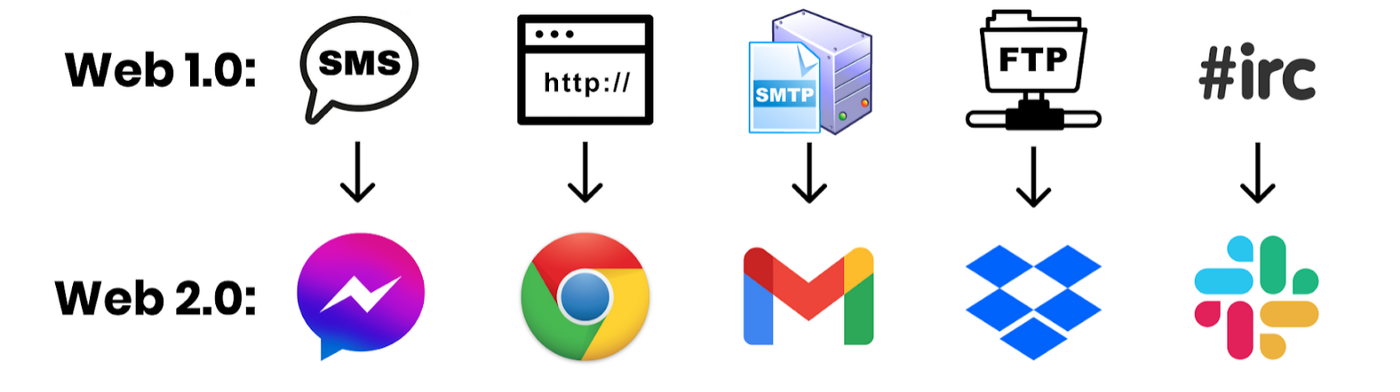
\includegraphics[width=\textwidth]{web_1_2.png}}
{Web 2 build on top of the open protocols of Web 1, aggregating user data and creating an easy-to-use, simple user experience.}


\Gls{web3}, unlike \gls{web2}, has a \gls{decentralized} distributed system. That means that all the nodes on the system in \gls{web3} have equal control and access. One of the key features of \gls{web3} is that it implements \gls{smart contract} and Token using the \gls{blockchain} mechanism. \\[-8pt]

At its core, Web 3 aims to allow users to not only read and write content but also own their own content so that they can’t get de-platformed or demonetized by centralized tech companies. Web 3 also aims to revert back to the open-source protocols of Web 1 where the rules are standardized for all market participants so that large tech companies can’t stifle innovation and market competition. \\[-8pt]